\documentclass[a4paper]{article}
\usepackage[english]{babel}
\usepackage[utf8]{inputenc}
\usepackage{textcomp}
\usepackage{amsmath}
\usepackage{gensymb}
\usepackage{physics}
\usepackage{graphicx}
\usepackage[colorinlistoftodos]{todonotes}
\usepackage[dvipsnames]{xcolor}
\usepackage{array}
\usepackage{tabularx}
\usepackage{tikz}
\usepackage{pgfplots}
\usepackage{framed}
\usepackage{xfrac}
\usepackage[most]{tcolorbox}
\usepackage{fix-cm}
\usepackage[margin=0.5in]{geometry}
\usetikzlibrary{quotes,angles}
\usetikzlibrary{decorations.pathreplacing}
\usetikzlibrary{calc}
\usepgfplotslibrary{fillbetween}

\let\phi\varphi
\let\bf\textbf
\colorlet{shadecolor}{orange!15}
\newcommand*{\comb}[2]{{}^{#1}C_{#2}}%
\pgfplotsset{compat=1.18}

\begin{document}
\section{Chapter 1}
\subsection{Types of data}
\begin{itemize}
    \item \bf{Nominal} - Qualitative only, cannot be arranged in order or ranked.
    \item \bf{Ordinal} - Qualitative or quantitative, can be arranged or ranked, but differences between data entries are not meaningful.
    \item \bf{Interval} - Quantitative only, can be ordered and meaningful differences between data entries can be calculated. Zero represents a position on a scale but \underline{not} an inherent zero.
    \item \bf{Ratio} - Quantitative only, can be ordered \& meaningful differences between data entries can be calculated. Zero \underline{does} represent an inherent zero.
\end{itemize}

\subsection{Sampling methods}
\begin{itemize}
    \item \bf{Simple random sample} - Every possible member of the population has an equal chance of being selected.
    \item \bf{Stratified sample} - Members of the population are divided into two or more subsets (strata) by a characteristic. A sample is then randomly selected from each of the strata, ensuring that all strata are sampled in proportion to their actual percentages of occurence in the population.
    \item \bf{Cluster sample} - Divide the population into groups (clusters) and select \underline{all} of the members in one or more (but not all) of the clusters. All clusters should have similar characteristics. Selecting all members of a population is called a census.
    \item \bf{Systematic sample} - Members of the population are selected at regular intervals from a randomly determined starting point.
\end{itemize}

\section{Chapter 2}
A \bf{frequency distribution} is a table that shows classes or intervals of data entries with a count of the umber of entries in each class.

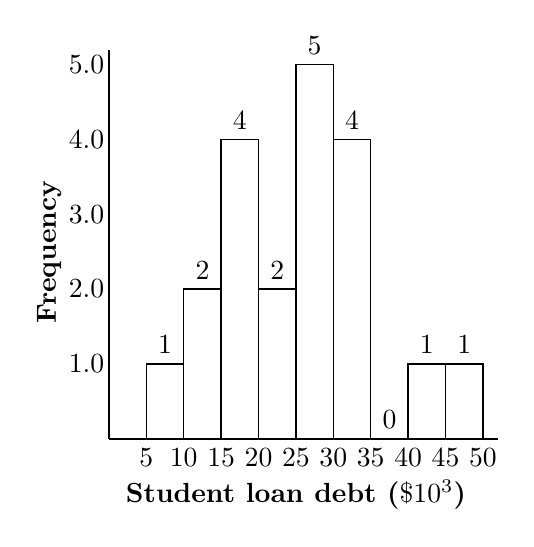
\begin{tikzpicture}[scale=0.95]
    %%% FREQUENCY DISTRIBUTION %%%
    % axes and labels %
    \draw[-,thick] (0,0)--(0,5.2);
    \draw[-,thick] (0,0)--(5.2,0);
    \node[rotate=90] at (-0.8,2.5){\bf{Frequency}};
    \node at (2.5,-0.75){\bf{Student loan debt ($\$10^3$)}};
    % y ticks %
    \node at (-0.3,1){1.0};
    \node at (-0.3,2){2.0};
    \node at (-0.3,3){3.0};
    \node at (-0.3,4){4.0};
    \node at (-0.3,5){5.0};
    % x ticks %
    \node at (0.5,-0.25){5};
    \node at (1,-0.25){10};
    \node at (1.5,-0.25){15};
    \node at (2,-0.25){20};
    \node at (2.5,-0.25){25};
    \node at (3,-0.25){30};
    \node at (3.5,-0.25){35};
    \node at (4,-0.25){40};
    \node at (4.5,-0.25){45};
    \node at (5,-0.25){50};
    % distribution %
    \draw[line width=0.5pt] (0.5,0)--(0.5,1)--node[above]{1}(1,1);
    \draw[line width=0.5pt] (1,0)--(1,2)--node[above]{2}(1.5,2);
    \draw[line width=0.5pt] (1.5,0)--(1.5,4)--node[above]{4}(2,4)--(2,2);
    \draw[line width=0.5pt] (2,0)--(2,2)--node[above]{2}(2.5,2);
    \draw[line width=0.5pt] (2.5,0)--(2.5,5)--node[above]{5}(3,5)--(3,4);
    \draw[line width=0.5pt] (3,0)--(3,4)--node[above]{4}(3.5,4)--(3.5,0);
    \draw[line width=0.5pt] (4,0)--(4,1)--node[above]{1}(4.5,1);
    \draw[line width=0.5pt] (4.5,0)--(4.5,1)--node[above]{1}(5,1)--(5,0);
    \node at (3.75,0.25){0};
\end{tikzpicture}

The class with the most data is called the modal class.
\subsection{Measures of central tendency}
\begin{itemize}
    \item \bf{Mean} - Sum of all sample values divided by the number of values: $\displaystyle\bar{x} = \frac{\sum x}{n}$
\end{itemize}
\vspace{2mm}
\begin{center}
    The weights in pounds of a sample of adults are listed here. Find the mean, median, and mode.\vspace{2mm}\\
    274, 235, 223, 268, 290, 285, 235
    \vspace{3mm}\\
    $\displaystyle\bar{x} = \frac{274 + 235 + 223 + 268 + 290 + 285 + 235}{7} = \frac{1810}{7} \approx 258.6$
\end{center}

\begin{itemize}
    \item \bf{Median} - The middle number of the data set when ordered smallest to largest (268). If the sample size is an even number, the median is the average of the two middle values.

    \item \bf{Mode} - The number that appears most in the data set. (235)

    \item The sample number is notated "$n$", the population number is "$N$". The mean of the sample is notated $\bar{x}$, the mean of the population is notated $\mu$.
\end{itemize}

\newpage
\subsection{Measures of variation and position}
Range = max - margin
\begin{itemize}
    \item \bf{Population Variance} - $\displaystyle\sigma^2 = \frac{\sum (x - \mu)^2}{N}$
    \item \bf{Sample Variance} - $\displaystyle s^2 = \frac{\sum (x - \bar{x})^2}{n - 1}$
    \item \bf{Population Standard Deviation} - $\displaystyle\sigma = \sqrt{\sigma^2}$
    \item \bf{Sample Standard Deviation} - $\displaystyle s = \sqrt{s^2}$
\end{itemize}
\bf{Empirical Rule} - Estimates the proportion of data within 1, 2, or 3 standard deviations of the mean.\\
\bf{Chebyshev's Theorem} - The proportion of any data set lying within $k$ standard deviations of the mean is \underline{at least} 
\begin{equation}
    1 - \frac{1}{k^2}
\end{equation}
\bf{Percentiles} - For any set of n measurments (arranged in ascending or descending order), the $p^{th}$ percentile means that $p\%$ of the measurments fall below the number and $(100 - p)\%$ fall above it.
\vspace{2mm}\\
\bf{Quartiles}
\begin{itemize}
    \item \bf{First Quartile} - About $\frac{1}{4}$ or $25\%$ of the data fall on or below the first quartile ($25^{th}$ percentile)
    \item \bf{Second Quartile} - About $\frac{1}{2}$ or $50\%$ of the data fall on or below the second quartile ($50^{th}$ percentile, median)
    \item \bf{Third Quartile} - About $\frac{3}{4}$ or $75\%$ of the data fall on or below the third quartile ($75^{th}$ percentile)
\end{itemize}
\bf{Interquartile Range} - The spread of the middle half of the data.
\vspace{2mm}\\
\bf{Identifying Outliers} 
\begin{itemize}
    \item Multiply IQR by 1.5 and subtract that value from Q1. Any data entry less than Q1 - 1.5(IQR) is an outlier. 
    \item Add 1.5(IQR) to Q3, any data entry greater than Q3 + 1.5(IQR) is an outlier
\end{itemize}
\bf{Z score} - The number of standard deviations a value $x$ lies from the mean ($\bar{x}$)
\begin{itemize}
    \item Sample z-score: $\displaystyle z = \frac{x - \bar{x}}{s}$
    \item Population z-score: $\displaystyle z = \frac{x - \mu}{\sigma}$
\end{itemize}

\section{Chapter 3}
\subsection{Probability, Combinations, Complements, Unions \& Intersections}
\bf{Sample Space} - The set of all sample points of an experiment. The sample space for tossing a die is:
\begin{equation}
    S = {1, 2, 3, 4, 5, 6}
\end{equation}
\bf{Event} - Subset of the sample space.
\vspace{5mm}\\
\bf{Probability Rules for Sample Points}\\
Let $p_i$ represent the probability of sample point $i$, then:
\begin{itemize}
    \item All sample point probabilities must lie between 0 and 1. $(0 \leq p_i \leq 1)$
    \item The probability of all the sample points within a sample space must sum to one. $\big(\sum p_i = 1\big)$
\end{itemize}
\vspace{5mm}
\bf{Types of Probability}
\begin{itemize}
    \item \bf{Classical (theoretical) probability} - Used when each outcome in a sample space is equally likely to occur. The classical probability for an event E is given by:
\end{itemize}
\begin{equation}
    P(E) = \frac{\text{number of outcomes in event $E$}}{\text{total number of outcomes in sample space}}
\end{equation}
\begin{itemize}
    \item \bf{Empirical (statistical) probability} - Based on observations obtained from probability experiments. The empirical probability of an event E is the relative frequency of event E.
\end{itemize}
\begin{equation}
    P(E) = \frac{\text{frequency of event $E$}}{\text{total frequency}} = \frac{f}{n}
\end{equation}
%%% missing some stuff 7/1 %%%
\newpage
\subsection{Combinations \& Complements}
\bf{Complement of Event} - The complement of an event is the set of all outcomes in a sample space that are \underline{not} included in event $E$
\begin{equation}
    P(E)^c = 1 - P(E) \ \to \ P(E) + P(E)^c = 1
\end{equation} 
\bf{Combinations Rule} - For a sample of $n$ elements to be drawn without replacement from a set of $N$ elements, the number of different samples is denoted by $\binom Nn$ and defined by: \hspace{15mm}(note $0! = 1$)
\begin{equation}
    \binom Nn = \frac{N!}{n!(N-n)!}
\end{equation}

\begin{shaded}
    \underline{\bf{Example:} The Lottery}
    \vspace{2mm}\\
    The Florida Lotto game consists of randomly selecting 6 numbers from the integers 1-53, a player who matches the 6 numbers wins the jackpot.
    \begin{itemize}
        \item[a)] Calculate the number of combinations for this drawning\\
        $\displaystyle \binom{53}{6} = \frac{53!}{6!(53-6)!} = \frac{53!}{6!\ 47!} = \frac{53 \cdot 52 \cdot 51 \cdot 50 \cdot 49 \cdot 48 \cdot 47!}{6 \cdot 5 \cdot 4 \cdot 3 \cdot 2 \cdot 1 \cdot 47!} = \frac{53 \cdot 52 \cdot 51 \cdot 50 \cdot 49 \cdot 48}{6 \cdot 5 \cdot 4 \cdot 3 \cdot 2 \cdot 1} = \frac{16,529,385,600}{720} = 22,957,480$ possible combinations
        \item[b)] What is the probability of winning the jackpot if you buy one ticket\\
        $\displaystyle P(\text{win}) = \frac{1}{22957480} = 4.356 \cdot 10^{-6}\ \%$
    \end{itemize}
\end{shaded}
\begin{shaded}
    \underline{\bf{Example:} Sock Drawer}
    \vspace{2mm}\\
    Your sock drawer contains 3 white socks and 2 black socks. In a hurry you randomly select socks from the drawer to wear to school.
    \begin{enumerate}
        \item List the sample points\\
        Sample points\\
        A$\
        \begin{cases}
            W_1,W_2\\
            W_2,W_3\\
            W_1,W_3
        \end{cases}$
        \vspace{1mm}\\
        B$\
        \begin{cases}
            W_1,B_1\\
            W_1,B_2\\
            W_2,B_1\\
            W_2,B_2\\
            W_3,B_1\\
            W_3,B_2
        \end{cases}$
        \vspace{1mm}\\
        C$\
        \begin{cases}
            B_1,B_2
        \end{cases}$
        \vspace{1mm}\\
        D = A + C
        \item Assign probabilities to the sample points\\
        Each sample point has a $\sfrac{1}{10}$ chance of being selected since the selection is random
        \item Determine the probabilities for each of the following events:
        \begin{itemize}
            \item[A:] \{Two white socks are selected\}
            \item[B:] \{One white sock \& one black sock are selected\}
            \item[C:] \{Two black socks are selected\}
            \item[D:] \{Matching socks are selected\} 
        \end{itemize}
        $P(A) = \sfrac{3}{10},\ \ P(B) = \sfrac{6}{10},\ \ P(C) = \sfrac{1}{10},\ \ P(D) = P(A) + P(C) = \sfrac{4}{10}$
    \end{enumerate}
\end{shaded}

\newpage
\subsection{Unions \& Intersections}
\bf{Fundamental Counting Principle} - If one event can occur $m$ ways, and another can occur $n$ ways, then the number of ways the two events can occur in sequence is $m \cdot n$. This can be extended to any number of events occuring in sequence.
\begin{shaded}
    \underline{\bf{Example:} License Plates}
    \vspace{2mm}\\
    How many license plates can be made consisting of 3 letters followed by 1 number?\\
    (\# of letters) $\cdot$ (\# of letters) $\cdot$ (\# of letters) $\cdot$ (\# numbers 0-9) $= (26)^3 \cdot 10 = 175,760$
\end{shaded}
\noindent\bf{Compound Event} - An event that can often be viewed as a composition of two or more events. There are two types of compound events:
\begin{itemize}
    \item \bf{Union} - The union of two events $A$ and $B$ is the event that occurs if either $A$ or $B$ (or both) occurs on a single performance of the experiment. The union of events $A$ and $B$ is denoted by $A \cup B$\\ $A \cup B$ consists of all the sample points that belong to \underline{$A$ or $B$ or both.}
    \item \bf{Intersection} - The intersection of two events $A$ and $B$ is the event that occurs if both $A$ and $B$ occur on a single performance of the experiment. The intersection of $A$ and $B$ is denoted $A \cap B$\\ $A \cap B$ consists of all the sample points belonging to \underline{both $A$ and $B$.}
\end{itemize}
\begin{shaded}
    \underline{\bf{Example:} Tossing Dice}
    \vspace{2mm}\\
    Consider a die-toss experiment in which the following events are defined:
    \begin{itemize}
        \item[A:] \{Toss an even number\} $(2,4,6)$
        \item[B:] \{Toss a number less than or equal to 3\} $(1,2,3)$  
    \end{itemize}
    \vspace{0.5mm}
    \begin{enumerate}
        \item Describe $A \cup B$ for this experiment\\
        $A \cup B$ is the event that a $1, 2, 3, 4,$ or $6$ is rolled.
        \item Describe $A \cap B$ for this experiment\\
        $A \cap B$ is the event that a $2$ is rolled
        \item Calculate $P(A \cup B)$ and $P(A \cap B)$\\
        $P(A \cup B) = \sfrac{5}{6},\ \ P(A \cap B) = \sfrac{1}{6}$
    \end{enumerate}
\end{shaded}

\begin{shaded}
    \underline{\bf{Example:} Streamer Preference}
    \vspace{2mm}\\
    A statistics student reported on a study of UCF students’ preference for either Netflix or Hulu. The study investigated the link between students’ preference and classification. The percentage of the surveyed students’ preference and classification is given in the table here
    \vspace{1mm}\\
    \begin{tabularx}{0.8\textwidth}{ 
        | >{\raggedright\arraybackslash}X 
        | >{\centering\arraybackslash}X 
        | >{\centering\arraybackslash}X | }
        \hline
        \bf{Classification} & \bf{Prefers Netflix} & \bf{Prefers Hulu} \\
        \hline
        Freshman & $10\%$ & $17\%$ \\
        \hline
        Sophomore & $14\%$ & $15\%$ \\
        \hline
        Junior & $13\%$ & $6\%$ \\
        \hline
        Senior & $22\%$ & $3\%$ \\
        \hline
    \end{tabularx}
    \vspace{1mm}\\
    Consider the Following definitions:
    \begin{itemize}
        \item[A:] \{Student prefers Netflix\}
        \item[B:] \{Student is a sophomore\} 
    \end{itemize}
    \begin{enumerate}
        \item Describe $A \cup B$ for this experiment\\
        $A \cup B$ is the event that a student prefers Netflix or is a sophomore or both
        \item Describe $A \cap B$ for this experiment\\
        $A \cap B$ is the event that a student is a sophomore who prefers Netflix
        \item Calculate $P(A \cup B)$ and $P(A \cap B)$\\
        $P(A \cup B) = 10\% + 14\% + 13\% + 22\% + 15\% = 74\%$ or 0.74\\
        $P(A \cap B) = 14\%$ or 0.14
    \end{enumerate}
\end{shaded}
\subsection{The Additive Rule and Mutually Exclusive Events}
\bf{Mutually Exclusive Events} - Events that cannot happen at the same time. Two events $A$ and $B$ are mutally exclusive when $A$ and $B$ cannot occur in a single performance of the experiment, that is, when $P(A \cap B) = 0$. The probability that mutually exclusive events $A$ or $B$ will occur is given by: \hspace{10mm} *(only for mutually exclusive events)*
\begin{equation}
    P(A \cup B) = P(A) + P(B)
\end{equation}
\begin{shaded}
    \underline{\bf{Example:} Blood Bank}
    \vspace{2mm}\\
    A blood bank catalogs the types of blood, including positive or negative Rh-factor, given by donors during the last five days. The number of donors who gave is shown in the table below.
    \vspace{1mm}\\
    \begin{tabularx}{0.6\textwidth}{ 
        | >{\raggedright\arraybackslash}X 
        | >{\centering\arraybackslash}X 
        | >{\centering\arraybackslash}X 
        | >{\centering\arraybackslash}X 
        | >{\centering\arraybackslash}X 
        | >{\centering\arraybackslash}X | }
        \hline
        & O & A & B & AB & Total \\
        \hline
        Positive & 156 & 139 & 37 & 12 & 344 \\
        \hline
        Negative & 28 & 25 & 8 & 4 & 65 \\
        \hline
        Total & 184 & 164 & 45 & 16 & 409 \\
        \hline
    \end{tabularx}
    \begin{enumerate}
        \item Find the probability that a donor has O bold\\
        $P(O) = \sfrac{184}{409} = 0.45 = 45\%$
        \item Find the probability that a donor has type A or type AB blood (mutually exclusive events)\\
        $P(A \cup AB) = P(A) + P(AB) = \sfrac{164}{409} + \sfrac{16}{409} = \sfrac{180}{409} = 0.44 = 44\%$
        \item Find the probability that a donor does not have positive Rh-factor\\
        $P(+)^c = 1 - P(+) = P(-), \hspace{2mm}\boldsymbol{\to}\hspace{2mm} 1 - \sfrac{344}{409} = \sfrac{65}{409} = 0.159 = 15.9\%$
        \item Find the probability that a donor has AB blood \underline{or} negative Rh-factor\\
        $P(AB \cup -) = P(AB) + P(-) - P(AB \cap -) = \sfrac{16}{409} + \sfrac{65}{409} - \sfrac{4}{409} = \sfrac{77}{409} = 0.188 = 18.8\%$
        \item Find the probability that a donor has O blood \underline{or} positive Rh-factor\\
        $P(O \cup +) = P(O) + P(+) - P(O \cap +) = \sfrac{184}{409} + \sfrac{344}{409} - \sfrac{156}{409} \sfrac{372}{409} \approx 0.91 = 91\%$
    \end{enumerate}
\end{shaded}

\noindent\bf{The Addition Rule} - The union of two events that are not mutually exclusive. In general, the probability that events $A$ or $B$ will occur is given by:
\begin{equation}
    P(A \cup B) = P(A) + P(B) - P(A \cap B)
\end{equation}
\begin{shaded}
    \underline{\bf{Example:} Cats vs. Dogs}
    \vspace{2mm}\\
    An instructor asks 35 of her students the following questions:
    \begin{itemize}
        \item Do you have a cat? 12 students said yes
        \item Do you have a dog? 22 students said yes
        \item Do you have both a cat and a dog? 6 students said yes
    \end{itemize}
    \vspace{1mm}
    Let $A$ = \{Student has a cat\} and $B$ = \{Student has a dog\}\\
    One of these students is chosen at random,
    \begin{enumerate}
        \item What is the probability the student has a cat?\\
        $P(A) = \sfrac{12}{35} = 0.343 = 34.4\%$
        \item What is the probability the student has a dog?\\
        $P(B) = \sfrac{22}{35} = 0.629 = 62.9\%$
        \item What is the probability the student has a cat or dog?\\
        $P(A \cup B) = P(A) + P(B) - P(A \cap B) = \sfrac{12}{35} + \sfrac{22}{35} - \sfrac{6}{35} = \sfrac{28}{35} = 0.8 = 80\%$
        \item What is the probability the student has neither a dog or a cat?\\
        $P(A \cup B)^c = 1 - P(P \cup B) = 1 - \sfrac{28}{35} = \sfrac{7}{35} = 0.2 = 20\%$
    \end{enumerate}
\end{shaded}

%%% ADD MISSING INFO FROM 7/2 LECTURE %%%
\subsection{The Multiplicative Rule \& Independent Events}
\bf{Independent Events} - Two events are independent when the occurence of one of the events does not affect the probability of the occurence of the other event. That is, when $P(B|A) = P(B)$
\vspace{2mm}\\
\noindent\bf{Multiplication Rule} - To find the probability of two independent events $A$ and $B$ occuring in sequence, use the rule:
\begin{equation}
    P(A \cap B) = P(A) \cdot P(B)
\end{equation}
\noindent If $P(A | B) = P(B)$, then  $A$ and $B$ are independent. If $A$ and $B$ are independent, then $P(A \cap B) = P(A) \cdot P(B)$
\subsection{Dependent Events \& Conditional Probability}
\bf{Conditional Probability} - The probability of an event occuring, given that another event has already occurred. The conditional probability of event $B$ occurring, given that event $A$ has occured, is denoted by $P(B|A)$. The probability that two events $A$ and $B$ will occur in sequence is $P(A \cap B) = P(A) \cdot P(B|A)$
\begin{equation}
    P(A|B) = \frac{P(A \cap B)}{P(B)}
\end{equation}

\section{Chapter 4}
\subsection{Two Types of Random Variables}
\bf{Random Variables} - A random variable $x$ represents a numerical value associated with each outcome of a probability experiment. There are two types of random variables: discreet and continuous.
\begin{itemize}
    \item \bf{Discreet} - The variable has a \underline{finite or countable} number of possible outcomes that \underline{can be listed}.
    \item \bf{Continuous} - The variable has an \underline{uncountable} number of possible outcomes, represented by an interval on a number line.
\end{itemize}
\subsection{Probability Distributions for Discreet Random Variables}
A complete description of a discreet random variable requires that we specify all values the random variable can assume, and the probability associated with each value.
\vspace{3mm}\\
\bf{Requirements for the probability distribution of a discreet random variable $x$}
\begin{itemize}
    \item $0 \leq P(x) \leq 1,\ $ The probability of $x$ must be between 0 and 1
    \item $\sum P(x) = 1,\ $ The sum of the probabilities of $x$ equals 1
\end{itemize}
\subsection{Expected Values of Discrete Random Variables}
The \bf{mean}, or \bf{expected value} of a discreet random variable $x$ is given by: \hspace{15mm} (same as weighted mean)
\begin{equation}
    \mu = E(x) = \sum x P(x)
\end{equation}
To calculate variance 
\begin{equation}
    \sigma^2 = \sum \big[x^2 P(x)\big] - \mu^2
\end{equation}
\subsection{The Binomial Random Variable}
\bf{Binomial Experiment} - A probability experiment that satisfies these conditions:
\begin{enumerate}
    \item The experiment has a fixed number of trials, where each trial is independent of the other trials.
    \item There are only two possible outcomes of interest for each trial. Each outcome can be classified as success (S) or failure (F).
    \item The probability of success is the same for each trial.
    \item The random variable $x$ counts the number of successful trials.
\end{enumerate}
\bf{Binomial probability formula:}
\begin{equation}
    P(x) = \binom{n}{x}p^xq^{n-x}
\end{equation}
Where $p$ = probability of success on a single trial, $q = 1 - p$, $n$ = number of trials, $x$ = number of successes in $n$ trials, $n - x$ = number of failures in $n$ trials, and $\displaystyle\binom{n}{x} = \frac{n!}{x!(n-x)!}$
\begin{itemize}
    \item \bf{Mean:} $\displaystyle \mu = np$
    \item \bf{Variance:} $\displaystyle \sigma^2 npq$
    \item \bf{Standard Deviation:} $\displaystyle \sigma = \sqrt{npq}$
\end{itemize}
\newpage
\begin{shaded}
    \underline{\bf{Example:} Flower Genetics}
    \vspace{2mm}\\
    Suppose that cross fertilizing a red and white flower produces a colored (non-white) offspring 75\% of the time. You cross fertilize five pairs of red and white flowers to produce five offspring. You want to find the probability you get exactly 2 colored offspring. $P(x = 2)$
    \begin{itemize}
        \item What are the possible outcomes for $x$, the number of colored offspring?\\
        $x$ could be $0, 1, 2, 3, 4,$ or $5$
        \item What is the probability of cross-fertilizing a red and white flower and the offspring is colored?\\
        $p = 0.75 = 75\%$
        \item For each trial (each time you cross-fertilize a pair), there are two possible outcomes
        \begin{itemize}
            \item Success: Colored offspring
            \item Failure: White offspring
        \end{itemize}
        \item The probability of success, denoted $p$, is the same for each trial.\\
        $p = 0.75$
        \item The probability of failure, denoted $q$, is the complement of success.\\
        $q = 1 - p = 1 - 0.75 = 0.25$
        \item The trials are independent because the outcome of one cross-fertilization does not influence or affect the outcome of another
        \item What is the probability of getting exactly 2 colored offspring?\\
        \begin{tabularx}{0.7\textwidth}{ 
            | >{\hsize=0.25\hsize \centering\arraybackslash}X 
            | >{\hsize=0.75\hsize \centering\arraybackslash}X | }
            \hline
            Outcome & Probability \\
            \hline
            c c w w w & (0.75)(0.75)(0.25)(0.25)(0.25) = $(0.75)^2(0.25)^3$\\
            c w c w w & (0.75)(0.25)(0.75)(0.25)(0.25) = $(0.75)^2(0.25)^3$\\
            c w w c w & (0.75)(0.25)(0.25)(0.75)(0.25) = $(0.75)^2(0.25)^3$\\
            c w w w c & (0.75)(0.25)(0.25)(0.25)(0.75) = $(0.75)^2(0.25)^3$\\
            w c w w c & (0.25)(0.75)(0.25)(0.25)(0.75) = $(0.75)^2(0.25)^3$\\
            w c w c w & (0.25)(0.75)(0.25)(0.75)(0.25) = $(0.75)^2(0.25)^3$\\
            w c c w w & (0.25)(0.75)(0.75)(0.25)(0.25) = $(0.75)^2(0.25)^3$\\
            w w c w c & (0.25)(0.25)(0.75)(0.25)(0.75) = $(0.75)^2(0.25)^3$\\
            w w c c w & (0.25)(0.25)(0.75)(0.75)(0.25) = $(0.75)^2(0.25)^3$\\
            w w w c c & (0.25)(0.25)(0.25)(0.75)(0.75) = $(0.75)^2(0.25)^3$\\
            \hline
        \end{tabularx}
        \vspace{1mm}\\
        $P(x = 2)  = (0.75)^2(0.25)^3 = 0.0879$\\
        Using the binomial probability formula: $P(x = 2) = \binom{5}{2}(0.75)^2(0.25)^{5-2} = 0.0879$
    \end{itemize}
\end{shaded}

\begin{shaded}
    \underline{\bf{Example:} History Quiz}
    \vspace{2mm}\\
    A history quiz has 10 questions with answer options A, B, C, D, and E. You forgot to study for the quiz and randomly guess for each question. Let $x$ = the number of questions you get correct on the quiz
    \begin{enumerate}
        \item Write the sample space for $x$\\
        $x = \{0, 1, 2, 3, 4, 5, 6, 7, 8, 9, 10\}$
        \item Find $E(x)$ and interpret its value practically\\
        $\mu = E(x) = np\ \to \ (10)(0.2) = 2$
        \item Calculate the probability that of getting 3 correct\\
        $P(x = 3) = \binom{10}{3}(0.2)^3(0.8)^{10 - 3} = (120)(0.2)^3(0.8)^7 = 0.2013$
        \item Find the probability that $x = 6$\\
        $P(x = 6) = \binom{10}{6}(0.2)^6(0.8)^{10 - 6} = (210)(0.2)^6(0.8)^4 = 0.0055$
        \item Calculate the probability that you get no more than 3 questions correct\\
        For $P(x \leq 3)$ use the binomial table, $n = 10$, $p = 0.2$, $k = 3$. $\ \ P(x \leq 3) = 0.879$
        \item Is it likely that you pass? Calculate the probability that you pass the quiz (at least 70\%)\\
        $P(x \geq 7) = 1 - P(x \leq 6)$
    \end{enumerate}
\end{shaded}

\newpage

\section{Chapter 5}
\subsection{Normal Probability Distributions}
\bf{Normal Distribution} - Continuous probability distribution for a random variable $x$. The graph of a normal distribution is bell/mound shaped
\begin{itemize}
    \item The normal distribution is symmetric about its mean $\mu$
    \item Its spread is determined by the value of its standard deviation $\sigma$
\end{itemize}

\pgfmathdeclarefunction{gauss}{3}{%
  \pgfmathparse{1/(#3*sqrt(2*pi))*exp(-((#1-#2)^2)/(2*#3^2))}%
}
\begin{center}
    \begin{tikzpicture}[scale=1]
        \begin{axis}[
            no markers, 
            domain=0:6, 
            samples=100,
            ymin=0,
            axis lines*=left, 
            xlabel=,
            every axis y label/.style={at=(current axis.above origin),anchor=south},
            every axis x label/.style={at=(current axis.right of origin),anchor=west},
            height=5cm, 
            width=12cm,
            xtick=\empty, 
            ytick=\empty,
            enlargelimits=false, 
            clip=false, 
            axis on top,
            grid = major,
            hide y axis
        ]
            \addplot [very thick,black,name path=A] {gauss(x, 3, 1)};
            \pgfmathsetmacro\valueA{gauss(0.75,3,1)}
            \pgfmathsetmacro\valueB{gauss(1.5,3,1)}
            \pgfmathsetmacro\valueC{gauss(2.25,3,1)}
            \pgfmathsetmacro\valueM{gauss(3,3,1)}
            \draw [black] (axis cs:0.75,0) -- (axis cs:0.75,\valueA)
                (axis cs:5.25,0) -- (axis cs:5.25,\valueA);
            \draw [black] (axis cs:1.5,0) -- (axis cs:1.5,\valueB)
                (axis cs:4.5,0) -- (axis cs:4.5,\valueB);
            \draw [black] (axis cs:2.25,0) -- (axis cs:2.25,\valueC)
                (axis cs:3.75,0) -- (axis cs:3.75,\valueC);
            \draw [black!70!,dashed] (axis cs:3,0) -- (axis cs:3,\valueM);
            \draw [yshift=2cm,thick,latex-latex](axis cs:2.25, 0) -- node[above] {$0.683$} (axis cs:3.75, 0);
            \draw [yshift=1cm,thick,latex-latex](axis cs:1.5, 0) -- node[above] {$0.954$} (axis cs:4.5, 0);
            \draw [yshift=0.2cm,thick,latex-latex](axis cs:0.75, 0) -- node[above] {$0.954$} (axis cs:5.25, 0);
            
            \node[below] at (axis cs:0.75, 0) {$\mu - 3\sigma$};
            \node[below] at (axis cs:1.5, 0) {$\mu - 2\sigma$}; 
            \node[below] at (axis cs:2.25, 0) {$\mu - \sigma$}; 
            \node[below] at (axis cs:3, 0) {$\mu$}; 
            \node[below] at (axis cs:3.75, 0) {$\mu + \sigma$};
            \node[below] at (axis cs:4.5, 0) {$\mu + 2\sigma$};
            \node[below] at (axis cs:5.25, 0) {$\mu + 3\sigma$};

            \path[name path=B] 
                (axis cs:\pgfkeysvalueof{/pgfplots/xmin},0)--
                (axis cs:\pgfkeysvalueof{/pgfplots/xmax},0);
            \addplot[white!20!teal] fill between[of=A and B, soft clip={domain=2.25:3.75},];
            \addplot[gray!40!green] fill between[of=A and B, soft clip={domain=1.5:2.25},];
            \addplot[gray!40!green] fill between[of=A and B, soft clip={domain=3.75:4.5},];
            \addplot[red!80] fill between[of=A and B, soft clip={domain=0.75:1.5},];
            \addplot[red!80] fill between[of=A and B, soft clip={domain=4.5:5.25},];
            \addplot[violet!80] fill between[of=A and B, soft clip={domain=0:0.75},];
            \addplot[violet!80] fill between[of=A and B, soft clip={domain=5.25:6},];

            \addplot [very thick,black,name path=A] {gauss(x, 3, 1)};
        \end{axis}
    \end{tikzpicture}
\end{center}
\bf{Standard Normal Distribution} - A normal distribution with $\mu = 0$ and $\sigma = 1$. A random variable with a standard normal distribution, denoted by the symbol $z$, is called a standard normal variable
\begin{shaded}
    \underline{\bf{Example:} Bottled Drink Volume}
    \vspace{2mm}\\
    The average volume of liquid in a particular type of bottled drink is 500 mL with standard deviation 9 mL. The volume distribution is mound shaped.
    \begin{enumerate}
        \item[(a)] Using the empirical rule, what percent of drinks have a volume between 482 and 518 mL? Above 518 mL?
        \begin{center}
            \begin{tikzpicture}[scale=0.75]
                \begin{axis}[
                    no markers, 
                    domain=0:6, 
                    samples=100,
                    ymin=0,
                    axis lines*=left, 
                    xlabel=,
                    every axis y label/.style={at=(current axis.above origin),anchor=south},
                    every axis x label/.style={at=(current axis.right of origin),anchor=west},
                    height=5cm, 
                    width=12cm,
                    xtick=\empty, 
                    ytick=\empty,
                    enlargelimits=false, 
                    clip=false, 
                    axis on top,
                    grid = major,
                    hide y axis
                ]
                    
                    \addplot [very thick,black,name path=A] {gauss(x, 3, 1)};
                    \pgfmathsetmacro\valueA{gauss(1,3,1)}
                    \pgfmathsetmacro\valueB{gauss(2,3,1)}
                    \pgfmathsetmacro\valueC{gauss(3,3,1)}
                    \draw [gray] (axis cs:1,0) -- (axis cs:1,\valueA)
                        (axis cs:5,0) -- (axis cs:5,\valueA);
                    \draw [gray] (axis cs:2,0) -- (axis cs:2,\valueB)
                        (axis cs:4,0) -- (axis cs:4,\valueB);
                    \draw [gray] (axis cs:3,0) -- (axis cs:3,\valueC);
                    \draw [yshift=0.3cm, latex-latex](axis cs:1, 0) -- node [fill=orange!15] {$~95\%$} (axis cs:5, 0);
                    
                    \node[below] at (axis cs:1, 0) {482}; 
                    \node[below] at (axis cs:2, 0) {491}; 
                    \node[below] at (axis cs:3, 0) {500}; 
                    \node[below] at (axis cs:4, 0) {509};
                    \node[below] at (axis cs:5, 0) {518};

                    \path[name path=B] 
                        (axis cs:\pgfkeysvalueof{/pgfplots/xmin},0)--
                        (axis cs:\pgfkeysvalueof{/pgfplots/xmax},0);
                    \addplot[gray!60!green] fill between[of=A and B, soft clip={domain=0:1},];
                    \addplot[gray!60!green] fill between[of=A and B, soft clip={domain=5:6},];
                \end{axis}
            \end{tikzpicture}
        \end{center}
        About 95\% of drinks have a volume between 482 mL and 518 mL, and about 2.5\% have a volume above 518 mL
        \item[(b)] What is the probability that a randomly selected drink has a volume below 490 mL?
        \begin{enumerate}
            \item[1.] Set up probability: $P(x < 490)$
            \item[2.] Convert $x$ to $z$: $\displaystyle z = \frac{x - \mu}{\sigma} = \frac{490 - 500}{9} = -1.11$
            \item[3.] Use z-table: $\displaystyle P(x < 490) = P(z < -1.11) = 0.1335$
            \begin{center}
                \begin{tikzpicture}[scale=0.75]
                    \begin{axis}[
                        no markers, 
                        domain=0:6, 
                        samples=100,
                        ymin=0,
                        axis lines*=left, 
                        xlabel=,
                        every axis y label/.style={at=(current axis.above origin),anchor=south},
                        every axis x label/.style={at=(current axis.right of origin),anchor=west},
                        height=5cm, 
                        width=12cm,
                        xtick=\empty, 
                        ytick=\empty,
                        enlargelimits=false, 
                        clip=false, 
                        axis on top,
                        grid = major,
                        hide y axis
                    ]
                        
                        \addplot [very thick,black,name path=A] {gauss(x, 3, 1)};
                        \pgfmathsetmacro\valueA{gauss(1,3,1)}
                        \pgfmathsetmacro\valueB{gauss(2,3,1)}
                        \pgfmathsetmacro\valueC{gauss(3,3,1)}
                        \draw [gray] (axis cs:1,0) -- (axis cs:1,\valueA)
                            (axis cs:5,0) -- (axis cs:5,\valueA);
                        \draw [gray] (axis cs:2,0) -- (axis cs:2,\valueB)
                            (axis cs:4,0) -- (axis cs:4,\valueB);
                        \draw [gray] (axis cs:3,0) -- (axis cs:3,\valueC);
                        %\draw [yshift=0.3cm, latex-latex](axis cs:1, 0) -- node [fill=orange!15] {$~95\%$} (axis cs:5, 0);
                        
                        \node[below] at (axis cs:1, 0) {482}; 
                        \node[below] at (axis cs:2, 0) {491}; 
                        \node[below] at (axis cs:3, 0) {500}; 
                        \node[below] at (axis cs:4, 0) {509};
                        \node[below] at (axis cs:5, 0) {518};
    
                        \path[name path=B] 
                            (axis cs:\pgfkeysvalueof{/pgfplots/xmin},0)--
                            (axis cs:\pgfkeysvalueof{/pgfplots/xmax},0);
                        \addplot[gray!60!green] fill between[of=A and B, soft clip={domain=0:1.98},];
                    \end{axis}
                \end{tikzpicture}
            \end{center}
        \end{enumerate}
        \item[(c)] What is the probability that a randomly selected drink has a volume above 475 mL?
        \vspace{1mm}\\
        $\displaystyle z = \frac{x - \mu}{\sigma} = \frac{475 - 500}{9} = -2.78$\\
        $\displaystyle P(x > 475) = P(z < -2.78) = 1 - 0.0027 = 0.9973$
        \begin{center}
            \begin{tikzpicture}[scale=0.75]
                \begin{axis}[
                    no markers, 
                    domain=0:6, 
                    samples=100,
                    ymin=0,
                    axis lines*=left, 
                    xlabel=,
                    every axis y label/.style={at=(current axis.above origin),anchor=south},
                    every axis x label/.style={at=(current axis.right of origin),anchor=west},
                    height=5cm, 
                    width=12cm,
                    xtick=\empty, 
                    ytick=\empty,
                    enlargelimits=false, 
                    clip=false, 
                    axis on top,
                    grid = major,
                    hide y axis
                ]
                    
                    \addplot [very thick,black,name path=A] {gauss(x, 3, 1)};
                    \pgfmathsetmacro\valueA{gauss(1,3,1)}
                    \pgfmathsetmacro\valueB{gauss(2,3,1)}
                    \pgfmathsetmacro\valueC{gauss(3,3,1)}
                    \draw [gray] (axis cs:1,0) -- (axis cs:1,\valueA)
                        (axis cs:5,0) -- (axis cs:5,\valueA);
                    \draw [gray] (axis cs:2,0) -- (axis cs:2,\valueB)
                        (axis cs:4,0) -- (axis cs:4,\valueB);
                    \draw [gray] (axis cs:3,0) -- (axis cs:3,\valueC);
                    %\draw [yshift=0.3cm, latex-latex](axis cs:1, 0) -- node [fill=orange!15] {$~95\%$} (axis cs:5, 0);
                    
                    \node[below] at (axis cs:1, 0) {482}; 
                    \node[below] at (axis cs:2, 0) {491}; 
                    \node[below] at (axis cs:3, 0) {500}; 
                    \node[below] at (axis cs:4, 0) {509};
                    \node[below] at (axis cs:5, 0) {518};

                    \path[name path=B] 
                        (axis cs:\pgfkeysvalueof{/pgfplots/xmin},0)--
                        (axis cs:\pgfkeysvalueof{/pgfplots/xmax},0);
                    \addplot[gray!60!green] fill between[of=A and B, soft clip={domain=0.5:6},];
                \end{axis}
            \end{tikzpicture}
        \end{center}
        \item[(d)] What is the probability that a randomly selected drink has a volume between 488 and 511 mL?
        \vspace{1mm}\\
        $\displaystyle z_1 = \frac{488 - 500}{9} = -1.33\ z_2 = \frac{511 - 500}{9} = 1.22$\\
        $P(488 < x < 511) = P(-1.33 < z < 1.22) = P(z < 1.22) - P(z < -1.33) = 0.8888 - 0.0918 - 0.7970$
        \begin{center}
            \begin{tikzpicture}[scale=0.75]
                \begin{axis}[
                    no markers, 
                    domain=0:6, 
                    samples=100,
                    ymin=0,
                    axis lines*=left, 
                    xlabel=,
                    every axis y label/.style={at=(current axis.above origin),anchor=south},
                    every axis x label/.style={at=(current axis.right of origin),anchor=west},
                    height=5cm, 
                    width=12cm,
                    xtick=\empty, 
                    ytick=\empty,
                    enlargelimits=false, 
                    clip=false, 
                    axis on top,
                    grid = major,
                    hide y axis
                ]
                    
                    \addplot [very thick,black,name path=A] {gauss(x, 3, 1)};
                    \pgfmathsetmacro\valueA{gauss(1,3,1)}
                    \pgfmathsetmacro\valueB{gauss(2,3,1)}
                    \pgfmathsetmacro\valueC{gauss(3,3,1)}
                    \draw [gray] (axis cs:1,0) -- (axis cs:1,\valueA)
                        (axis cs:5,0) -- (axis cs:5,\valueA);
                    \draw [gray] (axis cs:2,0) -- (axis cs:2,\valueB)
                        (axis cs:4,0) -- (axis cs:4,\valueB);
                    \draw [gray] (axis cs:3,0) -- (axis cs:3,\valueC);
                    %\draw [yshift=0.3cm, latex-latex](axis cs:1, 0) -- node [fill=orange!15] {$~95\%$} (axis cs:5, 0);
                    
                    \node[below] at (axis cs:1, 0) {482}; 
                    \node[below] at (axis cs:2, 0) {491}; 
                    \node[below] at (axis cs:3, 0) {500}; 
                    \node[below] at (axis cs:4, 0) {509};
                    \node[below] at (axis cs:5, 0) {518};

                    \path[name path=B] 
                        (axis cs:\pgfkeysvalueof{/pgfplots/xmin},0)--
                        (axis cs:\pgfkeysvalueof{/pgfplots/xmax},0);
                    \addplot[gray!60!green] fill between[of=A and B, soft clip={domain=1.67:4.22},];
                \end{axis}
            \end{tikzpicture}
        \end{center}
        \item[(e)] Suppose 200 drinks are selected. How many would you expect to have a volume between 488 and 511 mL?
        \vspace{1mm}\\
        $P(488 < x < 511) = 0.7970 \to (200)(0.7970) = 159.4$
    \end{enumerate}
\end{shaded}

\begin{shaded}
    \underline{\bf{Example:} Miles Per Gallon}
    \vspace{2mm}\\
    Suppose an auto manufacturer introduces a new model that has an advertised mean in-city mileage of 27 miles per gallon and standard deviation 3 mpg. Assume that the probability distribution of $x$, the in-city mileage for this car model can be approximated by the normal distribution with mean 27 mpg. ($\mu = 27, \sigma = 3$)
    \begin{enumerate}
        \item If you were to buy this model of automobile, what is the probability that you would purchase one that averages less than 20 mpg for in-city driving?
        \vspace{1mm}\\
        $\displaystyle z = \frac{x - \mu}{\sigma} = \frac{20 - 27}{3} = -2.33$
        \vspace{1mm}\\
        $P(x < 20) = P(z < -2.33) = 0.0099$
        \item Suppose you purchase one of these new models and it does get less than 20 mpg for in-city driving. Should you believe that the advertised mean is incorrect?
        \vspace{1mm}\\
        It is possible that you were just unlucky and got a car with gas mileage in the lower 0.99\% or the advertised mean could be incorrect and the true mean is lower than advertised 
    \end{enumerate}
\end{shaded}

\begin{shaded}
    \underline{\bf{General Normal Probability Examples}}
    \begin{enumerate}
        \item Find the probability that a standard normal random variable exceeds 1.64
        \vspace{1mm}\\
        For $P(z > n)$ use the complement of the probability from the table\\
        $P(z > 1.64) = 1 - 0.9495 = 0.0505$
        \item Find the probability that a standard normal random variable lies to the left of 0.67
        \vspace{1mm}\\
        For $P(z < n)$ use the probability from the table\\
        $P(z < 0.67) = 0.7486$
        \item Find the probability that a standard normal random variable falls between -1 and 2.5
        \vspace{1mm}\\
        For $P(n < z < m)$ look up both probabilities in the table and subtract the smaller probability from the larger probability\\
        $P(-1.00 < z < 2.50) = 0.9938 - 0.1587 = 0.8351$
    \end{enumerate}
\end{shaded}

\newpage
\begin{shaded}
    \underline{\bf{Example:} Newborn Weights}
    \vspace{2mm}\\
    Suppose that the weights of newborns in the US are normally distributed with a mean of 7 lbs and a standard deviation of 1.4 lbs.
    \begin{enumerate}
        \item What percent of babies' weights are above 6.2 lbs?
        \vspace{1mm}\\
        $\displaystyle z = \frac{x - \mu}{\sigma} = \frac{6.2 - 7}{1.4} = -0.57\ \boldsymbol{\to}\ P(x > 6.2) = P(z > -0.57) = 1 - 0.2843 = 0.7157$
        \begin{center}
            \begin{tikzpicture}[scale=1]
                \begin{axis}[
                    no markers, 
                    domain=0:6, 
                    samples=100,
                    ymin=0,
                    axis lines*=left, 
                    xlabel=,
                    every axis y label/.style={at=(current axis.above origin),anchor=south},
                    every axis x label/.style={at=(current axis.right of origin),anchor=west},
                    height=5cm, 
                    width=12cm,
                    xtick=\empty, 
                    ytick=\empty,
                    enlargelimits=false, 
                    clip=false, 
                    axis on top,
                    grid = major,
                    hide y axis
                ]
                    \addplot [very thick,black,name path=A] {gauss(x, 3, 1)};
                    \pgfmathsetmacro\valueA{gauss(0.75,3,1)}
                    \pgfmathsetmacro\valueB{gauss(1.5,3,1)}
                    \pgfmathsetmacro\valueC{gauss(2.25,3,1)}
                    \pgfmathsetmacro\valueM{gauss(3,3,1)}
                    \draw [black] (axis cs:0.75,0) -- (axis cs:0.75,\valueA)
                        (axis cs:5.25,0) -- (axis cs:5.25,\valueA);
                    \draw [black] (axis cs:1.5,0) -- (axis cs:1.5,\valueB)
                        (axis cs:4.5,0) -- (axis cs:4.5,\valueB);
                    \draw [black] (axis cs:2.25,0) -- (axis cs:2.25,\valueC)
                        (axis cs:3.75,0) -- (axis cs:3.75,\valueC);
                    \draw [black!70!,dashed] (axis cs:3,0) -- (axis cs:3,\valueM);
                    
                    \node[below] at (axis cs:0.75, 0) {2.8};
                    \node[below] at (axis cs:1.5, 0) {4.2}; 
                    \node[below] at (axis cs:2.25, 0) {5.6}; 
                    \node[below] at (axis cs:3, 0) {7}; 
                    \node[below] at (axis cs:3.75, 0) {8.4};
                    \node[below] at (axis cs:4.5, 0) {9.8};
                    \node[below] at (axis cs:5.25, 0) {11.2};

                    \node[below] at (axis cs:0.75, -0.05) {$\mu - 3\sigma$};
                    \node[below] at (axis cs:1.5, -0.05) {$\mu - 2\sigma$}; 
                    \node[below] at (axis cs:2.25, -0.05) {$\mu - \sigma$}; 
                    \node[below] at (axis cs:3, -0.05) {$\mu$}; 
                    \node[below] at (axis cs:3.75, -0.05) {$\mu + \sigma$};
                    \node[below] at (axis cs:4.5, -0.05) {$\mu + 2\sigma$};
                    \node[below] at (axis cs:5.25, -0.05) {$\mu + 3\sigma$};
        
                    \path[name path=B] 
                        (axis cs:\pgfkeysvalueof{/pgfplots/xmin},0)--
                        (axis cs:\pgfkeysvalueof{/pgfplots/xmax},0);
                    \addplot[white!20!teal] fill between[of=A and B, soft clip={domain=2.43:6},];
                    
                    \addplot [very thick,black,name path=A] {gauss(x, 3, 1)};
                \end{axis}
            \end{tikzpicture}
        \end{center}
        \item In a sample of 20 babies born today, how many would we expect to weigh above 6.2 lbs?
        \vspace{1mm}\\
        71.57\% are expected to weigh above 6.2 lbs, or $(20)(0.7157) = 14.314$
        \item A newborn baby's weight is 0.64 standard deviations above the mean, what is the baby's weight?
        \vspace{1mm}\\
        Use $z$ formula solved for $x$: $\displaystyle x = \mu + z\sigma$\\
        $x = 7 + (0.64)(1.4) =$ 7.896 lbs
        \item What is the largest weight a newborn can be to be considered in the lower 4.01\%?
        \vspace{1mm}\\
        Look on the negative side of the $z$ table for probability 0.0401 (-1.75)\\
        $x = \mu + z\sigma = 7 + (-1.75)(1.4) = 4.55$ lbs
        \item What is the smallest weight a newborn can be to be considered in the upper 2.68\%?
        \vspace{1mm}\\
        The cutoff for the upper 2.68\% is the lower 97.32\%. Look at the positive $z$ table for the probability 0.9732. ($z = 1.93$)\\
        $x = \mu + z\sigma = 7 + (1.93)(1.4) = 9.702$ lbs
    \end{enumerate}
\end{shaded}

\begin{shaded}
    \underline{\bf{General Examples of Finding $z$ Scores from a Probability/Cumulative Area}}
    \begin{enumerate}
        \item Find the $z$ score that corresponds to the cumulative area of 0.8554
        \vspace{1mm}\\
        Look on the positive side of the $z$ table for the probability 0.8554 ($z = 1.06$)\\
        $P(z < 1.06) = 0.8554$
        \item Find the $z$ score that corresponds to the 75th percentile
        \vspace{1mm}\\
        Look on the positive side of the $z$ table for the probability 0.7500 ($z = 0.67$)\\
        $P(z < 0.67) = 0.7500$
        \item Find the $z$ score that has 0.91\% of the distribution's area to its right
        \vspace{1mm}\\
        Look on the positive side of the $z$ table for the probability 0.9909 ($z = 2.36$)\\
        $P(z > 2.36) = 0.0091 = 1 - 0.9909$
        \item Find the $z$ score that corresponds to the 31st percentile
        \vspace{1mm}\\
        Look on the negative side of the $z$ table for the probability 0.3100, the closest is 0.3085. ($z = -0.50$)\\
        $P(z < -0.50) = 0.3100$
        \item Find the $z$ score for which 60\% of the distribution's area lies between $-z$ and $z$
        \vspace{1mm}\\
        Look on the negative side of the $z$ table for the probability 0.2000, the closest is 0.2005 ($z = \pm 0.84$). If the probability is \underline{exactly} between two probabilities in the table, average the two $z$ scores
        \vspace{0.5mm}\\
        $P(z_1 < x < z_2) = 0.6000\ \to\ P(-0.84 < x < 0.84)$
    \end{enumerate}
\end{shaded}

\begin{shaded}
    \underline{\bf{Example:} Find The Value of $x$ Given a Percentage}
    \vspace{2mm}\\
    The mean total cholesterol level of women ages 20-34 is 181 mg/dL with standard deviation 37.6 mg/dL. Assume the total cholesterol levels are normally distributed
    \begin{enumerate}
        \item What level represents the 99th percentile? Round to the nearest whole number
        \vspace{1mm}\\
        Look on the positive side of the $z$ table for the probability closest to 0.9900 (0.9901 is the closest). $z = 2.33$\\
        $x = \mu + z\sigma = 181 + (2.33)(37.6) = 269$ mg/dL
        \item What levels represent the bottom 10\%? Round to the nearest whole number
        \vspace{1mm}\\
        Look on the negative side of the $z$ table for the probability closest to 0.1000 (0.1003 is the closest). $z = -1.28$\\
        $x = \mu + z\sigma = 181 + (-1.28)(37.6) = 133$ mg/dL
        \item What level represents the third quartile? Round to the nearest whole number
        \vspace{1mm}\\
        The third quartile is the 75th percentile, look on the positive side of the $z$ table for the closest probability to 0.7500 (0.7486 is the closest). $z = 0.67$\\
        $x = \mu + z\sigma = 181 + (0.67)(37.6) = 206$ mg/dL
        \item What is the smallest cholesterol level to be considered in the top 15\%? Round to the nearest whole number
        \vspace{1mm}\\
        The top 15\% is the same as the 85th percentile, look on the positive side of the $z$ table for the probability closest to 0.8500 (0.8508 is the closest). $z = 1.04$\\
        $x = \mu + z\sigma - 181 + (1.04)(37.6) = 220$ mg/dL
    \end{enumerate}
\end{shaded}
\newpage

\section{Chapter 6}
\subsection{Sampling Distribution}
\bf{Sampling Distribution} - The probability distribution of a sample statistic that is formed when samples of size $n$ are repeatedly taken from a population
\vspace{1mm}\\
\bf{Properties of Sampling Distributions of Sample Means}
\begin{enumerate}
    \item The mean of the sample means $\mu_{\bar{x}}$ is equal to the population mean $\mu$
    \begin{align}
        \mu_{\bar{x}} = \mu
    \end{align}
    \item The standard deviation of the sample means $\sigma_{\bar{x}}$ (called the standard error of the mean) is equal to the population standard deviation $\sigma$ divided by the square root of the sample size $n$
    \begin{align}
        \sigma_{\bar{x}} = \frac{\sigma}{\sqrt{n}}
    \end{align}
\end{enumerate}
\subsection{Central Limit Theorem}
The central limit theorem states that:
\begin{enumerate}
    \item If samples of size $n$, where $n \geq 30$, are drawn from any population with a mean $mu$ and standard deviation $\sigma$, then the sampling distribution of the sample means approximates a normal distribution
    \item If the population itself is normally distributed, then the sampling distribution of sample means is normally distributed for any sample size $n$
\end{enumerate}

\end{document}